\section{Empirical Determination of Comparison Operations}

We empirically determine the number of comparisons between array elements for large, randomly generated arrays.
For Shellsort, we expect the runtime complexity to lie between $O(n\ \lg\ n)$ and $O(n^2)$.

To count the number of element comparisons, a counting variable $c_3$ can be employed, as illustrated in Listing~\ref{lst:shell}.
This variable increments each time an element comparison is performed.

Random arrays can be generated according to the method shown in Listing~\ref{lst:rand}, and the observed values of $c_3$ are recorded.
Since every comparison-based sorting algorithm belongs to the complexity class $\Omega(n\ \lg\ n)$, it is reasonable to assume that, on average, $c_3 \geq n\ \lg\ n$ holds (\cite[154]{OW17b}).\\









Early \textit{empirical} findings led \textit{Shell} to the assumption:

\blockquote[{\cite[31]{She59}}]{It appears that the time required to sort $n$ elements is proportional to $n^{1.226}$.
}

Naturally, these tests were constrained by small input sizes and the performance limitations of late 1950s hardware.

To avoid misinterpretations regarding the asymptotic upper bound of $O(n \log n)$, it is important to examine its growth behavior for varying $n$.
Notably, the inequality $n^{\frac{4}{3}} > n \log n$ holds for input sizes $n \geq 982$ (see Figure~\ref{fig:lognplot}).

\begin{figure}[!h]
    \centering
    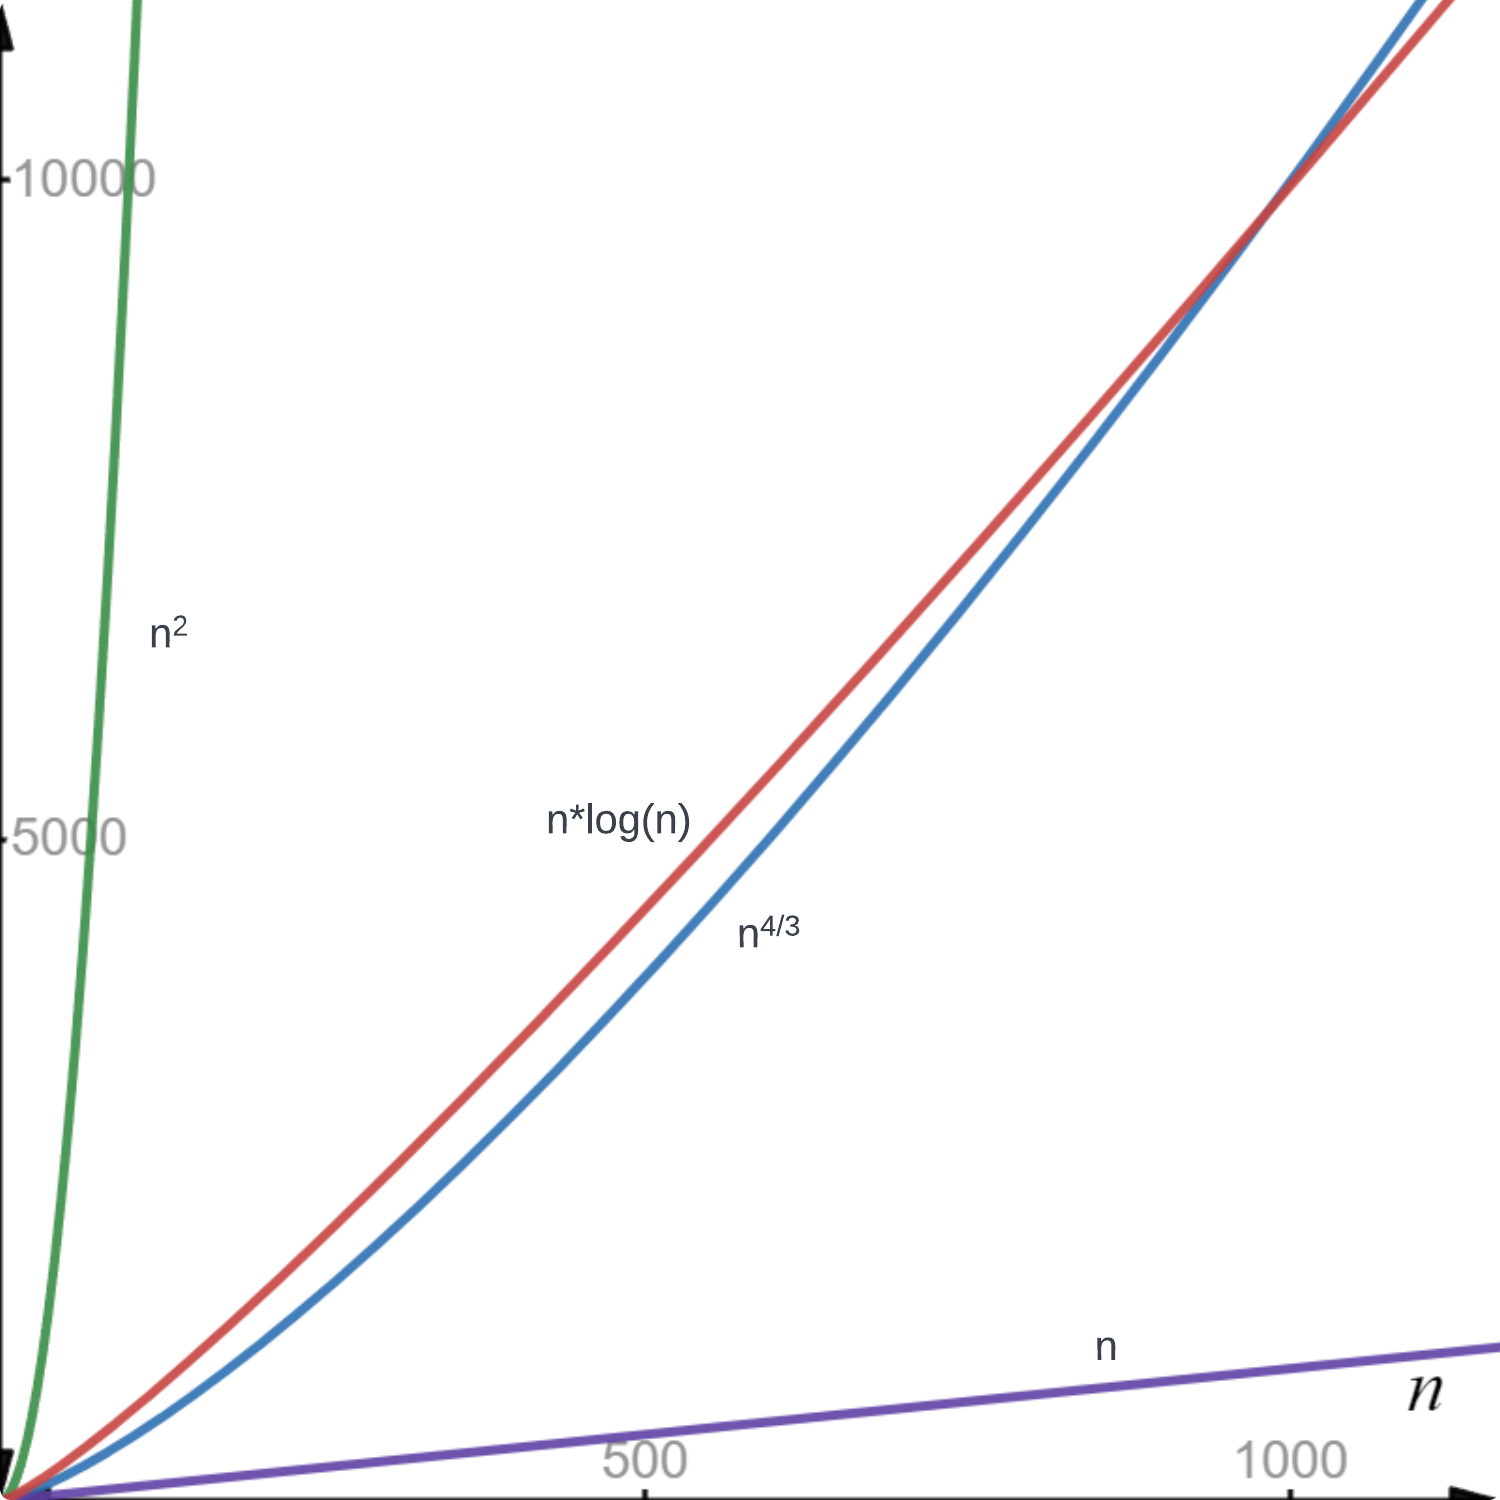
\includegraphics[width=0.8\columnwidth]{img/lognplot}
    \caption{For $n \geq 982$, $n^{\frac{4}{3}}$ grows faster than $n \log n$.}
    \label{fig:lognplot}
\end{figure}

This behavior must be carefully considered when interpreting empirical results for $n$.
Otherwise, one might incorrectly conclude that Shellsort achieves optimal runtime complexity of $O(n \log n)$, while in fact the observed upper bound of $O(n^{4/3})$ already exceeds $n \log n$ and approaches quadratic complexity for larger $n$.



\vspace{4mm}
\begin{lstlisting}[style=javastyle, caption={Code for Shellsort-testing large randomized arrays.}, label=lst:rand]
int epochs = 100;
while(epochs-- >= 0) {
    int[] tests = new int[]{
        2_000_000 /*, 4_000_000, ...*/
    };
    Random r = new Random();
    for (int i = 0; i < tests.length; i++) {
        int l = tests[i];
        int[] arr = new int[l];

        for (int j = l; j > 0; j--) {
            arr[l - j] = r.nextInt(l + 1);
        }

        ShellSort.sort(
            Arrays.copyOfRange(
                arr, 0, arr.length));
    }
}
\end{lstlisting}
\vspace{4mm}


\subsection{Test Results}

Test execution with large values of $n$ indicates that the number of comparisons $c_3$ falls either between $n\ \lg\ n$ and $n^{\frac{4}{3}}$, or between $n^{\frac{4}{3}}$ and $n^2$, depending on the input.
With a lower bound $\Omega(n\ \lg\ n)$ for all comparison-based sorting algorithms, we focus on the empirical comparison counts $c_3$ within

\begin{itemize}
    \item $n \lg\ n \leq c_3 < n^{\frac{4}{3}}$ \textit{(moderately efficient)}
    \item $n^{\frac{4}{3}} \leq c_3 \leq n^2$ \textit{(less efficient)}
\end{itemize}\\
\vspace{2mm}

With 100 epochs and array sizes up to $n = 2.000.000$, the test from Listing~\ref{lst:rand} yielded the following distribution of observed comparison counts $c_3$:

\begin{itemize}
    \item In 74 out of 100 cases, the measured $c_3$ satisfied $n^{\frac{4}{3}} < c_3 < n^2$.
    \item In 26 out of 100 cases, the measured $c_3$ lay between $n\ \lg\ n$ and $n^{\frac{4}{3}}$, i.e., $n\ \lg\ n < c_3 < n^{\frac{4}{3}}$.
\end{itemize}

These results support the hypothesis that Shellsort often exhibits sub-quadratic runtime behavior, but does not consistently remain within the $O(n\ \lg\ n)$ bound.



